\section{Zielsetzung}
\label{sec:Zielsetzung}
Das Ziel dieses Versuches ist es, Emissionsspektren einer Cu-Röntgenröhre und Absorptionsspektren verschiedener Materialien
aufzunehmen und zu analysieren.

\section{Theorie}
\label{sec:Theorie}

\subsection{Emission von Röntgenstrahlung} % (fold)
\label{sub:Emission}
Zur Erzeugung von Röntgenstrahlung wird eine Röntgenröhre verwendet.
In dieser werden aus einer Glühkathode durch den glühelektrischen Effekt Elektronen emittiert, welche durch ein elektrisches Feld beschleunigt
werden und dann auf eine Anode treffen. Beim Auftreffen auf die Anode kommt es zu einer starken Abbremsung, infolgedessen
Energie in Form von Röntgenstrahlung abgegeben wird.
Die entstandene Röntgenstrahlung wird unterteilt in das kontinuierliches Bremsspektrum und die charakteristische Röntgenstrahlung 
des Anodenmaterials.\\ 
Das kontinuierliche Bremsspektrum entsteht, weil das Elektron beim Auftreffen auf die Anode vom Coulombfeld des Atomkerns abgebremst
wird und dadurch ein Röntgenquant emittiert wird, dessen Energie dem Energieverlust des abgebremsten Elektron entspricht.
Durch die Tatsache, dass Elektronen ihre gesamte kinetische Energie oder nur einen Teil davon abgeben können, ist das Bremsspektrum
ein kontinuierliches Spektrum, welches in \autoref{fig:Abb_1} dargestellt ist.
\begin{figure}[H]
    \centering
    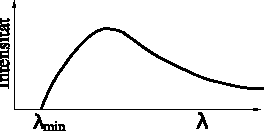
\includegraphics[width=0.3\textwidth]{build/Abb_1.pdf}
    \caption{Das kontinuierliche Spektrum der Bremsstrahlung.\cite{V602}}
    \label{fig:Abb_1}
\end{figure}
In dem Fall, dass das Elektron seine gesamte kinetische Energie $E_{kin}= e_0 U$ abgibt und diese in Strahlungsenergie $E = h \nu$ umgewandelt wird, ergibt
sich eine maximale Energie bzw. minimale Wellenlänge
\begin{align}
    \lambda_{min} &= \frac{h\cdot c}{e_0 U}, \label{eqn:lambdamin}
\end{align}
mit der Elementarladung $e_0$, der Beschleunigungsspannung $U$, des Planck'schen Wirkungsquantums $h$ und der Lichtgeschwindigkeit
im Vakuum $c$.\\

Das charakteristische Spektrum der Röntgenstrahlung entsteht durch die Ionisierung der Anode.
Hierbei ensteht in einer inneren Schale eine Lücke und ein Elektron von einer äußeren Schale kann unter Aussendung eines Röntgenquants
in die innere Schale zurückfallen. Die Energie des Röntgenquants entspricht hier der Energiedifferenz der beiden Energieniveaus der Schalen
$h \nu = E_m-E_n$. Somit besteht das charakteristische Spektrum aus scharfen Linien, welche mit $K_\alpha, K_\beta, L_\alpha$ bezeichnet werden,
abhängig davon auf welche Schale das Elektron zurückfällt. Die griechischen Indizes stehen für die Schale aus der das Elektron kommt.
Das Spektrum ist charakteristisch, da es sich um ein diskretes Spektrum handelt, das je nach Anodenmaterial verschieden ist.
In einem Atom mit mehreren Elektronen verringert sich durch die Wechselwirkungen der Elektronen die Coulomb-Anziehung auf die äußeren
Elektronen. Die Bindungsenergie eines Elektrons auf der nten Schale wird durch 
\begin{align}
    E_n &= -R_\infty z_{eff}^2 \cdot \frac{1}{n^2} \label{eqn:Bindungsenergie}
\end{align}
beschrieben, mit der Rydbergenergie $R_\infty = \qty{13.6}{\electronvolt}$ und der effektiven Kernladung $z_{eff} = z - \sigma$.
$\sigma$ ist die Abschirmkonstante, welche sich für jedes Elektron unterscheidet und empirisch bestimmbar ist.
Die Spektrumslinien der äußeren Elektronen teilen sich in mehrere eng aneinanderliegende Linien auf (Feinstruktur), da die äußeren
Elektronen aufgrund des Bahndrehimpulses und des Elektronenspins nicht alle dieselbe Bindungsenergie besitzen.
Die Energie der einzelnen Linien kann mithilfe der Sommerfeld'schen Feinstrukturformel
\begin{align}
    E_{n,j} &= -R_\infty \bigl(z_{eff,1}^2 \cdot \frac{1}{n^2} + \alpha^2 z_{eff,2}^4 \cdot \frac{1}{n^3} \bigl(\frac{1}{j+\frac{1}{2}} - \frac{3}{4n}\bigr)\bigr)
    \label{eqn:Sommerfeld}
\end{align}
bestimmt werden.
$\alpha = \frac{1}{137}$ ist hierbei die Sommerfeld'sche Feinstrukturkonstante, $n$ die Hauptquantenzahl und $j$ der Gesamtdrehimpuls des Elektrons.
Für die K-Schale gilt unter Vernachlässigung des Drehimpulses
\begin{align}
    E_{K,abs} &= R_\infty (z-\sigma_1)^2 \label{eqn:Ekabs}\\
    E_{K,\alpha} &= R_\infty \bigl(\frac{1}{n}\bigr)^2 \cdot (z-\sigma_1)^2 - R_\infty \bigl(\frac{1}{m}\bigr)^2 \cdot (z-\sigma_2)^2 \label{eqn:Eka}\\
    E_{K,\beta} &= R_\infty \bigl(\frac{1}{n}\bigr)^2 \cdot (z-\sigma_1)^2 - R_\infty \bigl(\frac{1}{l}\bigr)^2 \cdot (z-\sigma_3)^2. \label{eqn:Ekb}
\end{align}

% subsection Emission von Röntgenstrahlung (end)

\subsection{Absorption von Röntgenstrahlung} % (fold)
\label{sub:Absorption}

Besitzt die Röntgenstrahlung eine Energie, die kleiner ist als $\qty{1}{\mega\electronvolt}$, treten als dominante Prozesse bei der
Absorption der Compton-Effekt und der Photo-Effekt auf. Daher nimmt der Absorptionskoeffizient bei zunehmender Energie ab, wenn die
Röntgenstrahlung auf einen Absorber trifft, steigt jedoch sprunghaft an, sobald die Photoenenergie gerade größer ist als die
Bindungsenergie eines Elektrons aus der nächsten inneren Schale. Dieses Phänomen ist in \autoref{fig:Abb_2} dargestellt.
\begin{figure}[H]
    \centering
    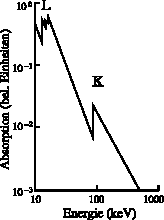
\includegraphics[width=0.2\textwidth]{build/Abb_2.pdf}
    \caption{Absorptionsverlauf in Abhängigkeit der Energie der Röntgenstrahlung.\cite{V602}}
    \label{fig:Abb_2}
\end{figure}
Die Energie der Elektronen und die Lage der Absorptionskante $E_n - E_\infty = h \nu_{abs}$ sind beinahe identisch. Die zugehörigen
Energien  werden Absorptionskanten genannt. Sie werden nach der Schale benannt wo das Elektron hergekommen ist.
Aufgrund der Feinstruktur gibt es drei L-Kanten, jedoch nur eine K-Kante.
Für die Elektronen der K-Schale kann aus der K-Kante mit der Sommerfeld'schen Feinstruktur (siehe \autoref{eqn:Sommerfeld}) die
Abschirmkonstante
\begin{align}
    \sigma_K &= Z - \sqrt{\frac{E_K}{R_\infty} - \frac{\alpha^2 Z^4}{4}} \label{eqn:sigmak}
\end{align}
bestimmt werden. $Z$ ist hier die Ordnungszahl des Absorbermaterials.
Die Berechnung der Abschirmkonstante der L-Kanten ist komplizierter.
Im Versuch ist die $L_I$ - und die $L_{II}$ -Kante jedoch nicht zu unterscheiden und es wird die Differenz $\Delta E_L = E_{L,II} - E_{L,III}$
verwendet.
Daher ergibt sich für die Abschirmkonstante der L-Schale
\begin{align}
    \sigma_L &=  Z - \Biggl(\frac{4}{\alpha} \sqrt{\frac{\Delta E_L}{R_\infty}}-\frac{5 \Delta E_L}{R_\infty}\Biggr)^{\frac{1}{2}}
    \Biggl(1 + \frac{19}{32} \alpha^2 \frac{\Delta E_L}{R_\infty} \Biggr)^{\frac{1}{2}}. \label{eqn:sigmal}
\end{align}

% subsection Absorption von Röntgenstrahlung (end)

\subsection{Analyse der Röntgenstrahlung} % (fold)
\label{sub:Analyse}

Analysieren lässt sich die Wellenlänge und somit auch die Energie der Röntgenstrahlung experimentell mithilfe der
Bragg'schen Reflexion.(siehe \autoref{fig:Abb_3})
\begin{figure}[H]
    \centering
    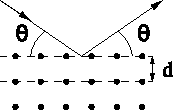
\includegraphics[width=0.3\textwidth]{build/Abb_3.pdf}
    \caption{Reflexion der Röntgenstrahlung am Gitterkristall.\cite{V602}}
    \label{fig:Abb_3}
\end{figure}
Die in der Röntgenröhre erzeugte Röntgenstrahlung fällt auf einen LiF-Kristall. An jedem Atom des Kristallgitters werden die
Photonen gebeugt. Die Röntgenstrahlen interferieren miteinander und bei einem bestimmten Winkel gibt es konstruktive Interferenz.
Dieser Winkel $\theta$ wird Glanzwinkel genannt.
Die Beziehung zwischen Glanzwinkel $\theta$, und gebeugter Wellenlänge $\lambda$ ist durch die Bragg-Bedingung
\begin{align}
    2 d \sin{\theta} = n \lambda \label{eqn:Bragg}
\end{align}
gegeben, wobei $d$ die Gitterkonstante und $n$ die Beugungsordnung ist.
% subsection Analyse der Röntgenstrahlung (end)